\documentclass[11pt,a4paper]{article}

\usepackage[margin=2.2cm]{geometry}
\usepackage{fontspec}
\usepackage{xcolor}
\usepackage{hyperref}
\usepackage{graphicx}
\usepackage{booktabs}
\usepackage{longtable}
\usepackage{array}
\usepackage{enumitem}
\usepackage{tabularx}
\usepackage{float}
\usepackage{titlesec}
\usepackage{xurl}
\usepackage{fvextra}
\usepackage{subcaption}

\setmainfont{Arial}
\graphicspath{{../report_assets/}{../results/}}
\hypersetup{colorlinks=true, linkcolor=blue, urlcolor=blue}
\setlist[itemize]{leftmargin=1.2em}
\setlist[enumerate]{leftmargin=1.4em}
\titleformat{\section}{\Large\bfseries}{\thesection}{0.6em}{}
\titleformat{\subsection}{\large\bfseries}{\thesubsection}{0.6em}{}
\DefineVerbatimEnvironment{verbatim}{Verbatim}{breaklines=true, breakanywhere=true, fontsize=\small}
\newcolumntype{Y}{>{\raggedright\arraybackslash}X}
\sloppy

\newcommand{\pending}[1]{\begingroup\setlength{\fboxsep}{2pt}\colorbox{yellow!55}{\parbox{\dimexpr\linewidth-2\fboxsep\relax}{\textbf{PENDING:} #1}}\endgroup}

\begin{document}
\begin{titlepage}
\centering
\vspace*{1.5cm}
{\Large Artificial Intelligence Group Assignment Report\par}
\vspace{1.3cm}
{\huge\bfseries Ticket Routing Intelligence\par}
\vspace{0.35cm}
{\large Explainable Multilingual Queue and Priority Prediction for Customer Support Triage\par}
\vspace{1.1cm}
{\large 36121 Artificial Intelligence Principles and Applications\par}
\vspace{0.35cm}
{\large AT3 -- Group 2\par}
\vspace{1cm}
\begin{tabularx}{0.82\linewidth}{Y r}
\toprule
\textbf{Group member} & \textbf{Student ID}\\
\midrule
Tumadhir Alsharhan & 25605852\\
Amal Maawadh & 25605864\\
Andres Ethorimn & 26029165\\
Laura Pacheco & 25940875\\
Mario Rubiano & 24900627\\
Carl Lazarus & 12043485\\
\bottomrule
\end{tabularx}
\vfill
\begin{tabularx}{0.82\linewidth}{>{\bfseries}p{0.28\linewidth} Y}
\toprule
Repository & \url{https://github.com/ETHLOB/trn-uts-aipa}\\
Prototype name & Ticket Routing Intelligence\\
Submission date & 16 May 2026\\
\bottomrule
\end{tabularx}
\vspace*{1cm}
\end{titlepage}

\tableofcontents
\newpage

\section{Executive Summary}
\subsection{Overview of the Project}
Ticket Routing Intelligence is an AI decision-support system for customer support ticket triage. The system analyses a customer ticket and returns five outputs: predicted queue/category, predicted priority, recommended support team, escalation flag, short summary, and explanation terms. The aim is not to replace human agents. The aim is to provide a structured first-pass recommendation so agents can review tickets faster and more consistently.

The implementation uses the Kaggle Multilingual Customer Support Tickets dataset. Five CSV files were audited. Three compatible multilingual files were merged, while two German-normalized files were excluded because their queue labels used a different taxonomy. After deduplication and filtering, the modelling dataset contains 44,275 usable tickets.

\subsection{Objectives}
The project objectives are:
\begin{itemize}
  \item predict support queue/category from ticket text and safe pre-resolution metadata;
  \item predict priority as high, medium, or low;
  \item compare explainable NLP classifiers using validation and test metrics;
  \item benchmark multilingual transformer embeddings as an alternative representation;
  \item add rule-based routing and escalation logic;
  \item provide human-readable summaries and explanation terms;
  \item present the solution through a Streamlit dashboard with single-ticket and batch-ticket analysis.
\end{itemize}

\subsection{Key Findings}
The selected model is TF-IDF with Linear SVM for both prediction tasks. On the held-out test set, it reached macro F1 of 0.525 for queue/category prediction and 0.568 for priority prediction. Billing and Payments was the strongest category with F1 around 0.779, and high priority reached F1 around 0.624. These results are useful for first-pass triage, but they do not support full automation. This finding supports a human-in-the-loop design.

An optional sampled transformer-embedding benchmark was also implemented using multilingual MiniLM sentence embeddings and Logistic Regression. It reached sampled macro F1 of 0.235 for category and 0.350 for priority. In the current setup, transformer embeddings did not outperform the full-data TF-IDF Linear SVM pipeline. This result is useful because it shows that a more complex AI representation is not automatically better without tuning, larger samples, and careful validation.

\section{Introduction}
\subsection{Background and Context}
Customer support teams receive large volumes of unstructured tickets. These tickets can mention billing problems, product questions, account access, service outages, returns, security concerns, or general requests. In real operations, first-pass triage is important because it decides which team receives the ticket and how fast it is reviewed. Manual triage can be slow and inconsistent, especially when tickets are multilingual or when urgent words are hidden inside long messages.

\subsection{Problem Statement}
The problem is slow and inconsistent ticket triage. A support ticket must be mapped to a queue, assigned a priority, checked for escalation risk, and routed to the correct team. If the first decision is wrong, customers wait longer and urgent cases can be missed. This project builds an AI prototype that assists this decision while keeping humans responsible for final action.

\subsection{Significance and Impact}
The system can reduce manual work by giving agents an initial recommendation. It can also improve transparency by showing explanation terms and escalation reasons. This is important because a support team should not rely on an unexplained prediction. The prototype also supports batch upload, so a team can analyse several tickets from a CSV or Excel file.

\subsection{Challenges and Constraints}
The main constraints are dataset imbalance, multilingual text, overlapping category language, and privacy. Some categories share similar words, such as product support and technical support. Some languages have fewer examples, which affects fairness. Also, ticket text may include personal information, so the summary function masks obvious email addresses and phone numbers. Finally, the project must stay reproducible for an academic assignment, so the deployed demo uses simple and explainable methods instead of external LLM services.

\subsection{Project Objectives and Scope}
The project scope is a working prototype and reproducible pipeline. It includes notebooks, reusable Python modules, saved metrics, charts, and a Streamlit app. It does not claim production readiness. A real deployment would need ticketing-system integration, access control, monitoring, retraining workflows, stronger privacy redaction, and testing on company-specific data.

\section{Theoretical Justification}
\subsection{Overview of AI Methods Used}
The solution combines several AI methods:
\begin{itemize}
  \item supervised NLP classification for queue and priority prediction;
  \item TF-IDF vectorisation to convert text into sparse numerical features;
  \item Logistic Regression, Naive Bayes, and Linear SVM as comparison models;
  \item rule-based reasoning for routing and escalation;
  \item template-based summarisation with privacy masking;
  \item explanation terms from influential TF-IDF features;
  \item optional multilingual transformer embeddings for comparison evidence.
\end{itemize}

\subsection{Theoretical Foundations}
TF-IDF gives high weight to words that are frequent in one document but less frequent across the full corpus. This is useful for support tickets because terms such as ``invoice'', ``refund'', ``outage'', or ``password'' can be strong signals for a queue. Linear SVM is suitable for sparse, high-dimensional text features because it learns a separating boundary between classes and often performs well for text classification. Logistic Regression gives a strong linear baseline with probabilistic interpretation, while Naive Bayes is a simple probabilistic baseline that is often used for text.

The rule-based layer represents operational knowledge. For example, if a ticket includes words such as ``unauthorised'', ``fraud'', or ``breach'', the app can recommend a security team or escalation review even if the predicted queue is not security. This combination is important because ML predictions and business rules solve different parts of the triage task.

\subsection{Justification of Selected Methods}
Linear SVM was selected because it had the best validation macro F1 for both queue and priority. It also keeps the system lightweight, fast, and explainable. The app can show influential TF-IDF terms, which helps agents understand the prediction. This approach is more suitable for the current prototype than a heavier model that is harder to run and explain.

The transformer benchmark was kept separate from live prediction. It provides a semantic multilingual comparison, but it used a sample of 2,500 tickets and performed below the current model. Therefore, it is report evidence and future-work evidence, not the deployed prediction path.

\subsection{Transformer Benchmark Rationale}
The transformer benchmark used the multilingual MiniLM sentence-transformer model to encode ticket text as dense multilingual sentence embeddings. A Logistic Regression classifier was then trained on those embeddings for the same two tasks: category prediction and priority prediction. This experiment was added because transformer embeddings are designed to capture semantic similarity across languages, which is relevant for a multilingual ticket dataset. However, it was intentionally run as a sampled benchmark because transformer inference is heavier than TF-IDF and was not required for the live demo.

\subsection{Related Work / Literature Support}
The project follows common NLP classification practice: text normalisation, TF-IDF feature extraction, train/validation/test splitting, model comparison, and held-out evaluation. The responsible AI design follows principles of human oversight, leakage control, transparency, and privacy minimisation.

\section{Workflow and Methodology}
\subsection{System Architecture Overview}
The workflow has seven main stages: audit data, prepare text, build features, train models, evaluate results, route tickets, and explain outputs. The Streamlit app presents this workflow in the Overview tab and provides prediction tools in the Try Solution tab.

\begin{figure}[H]
\centering
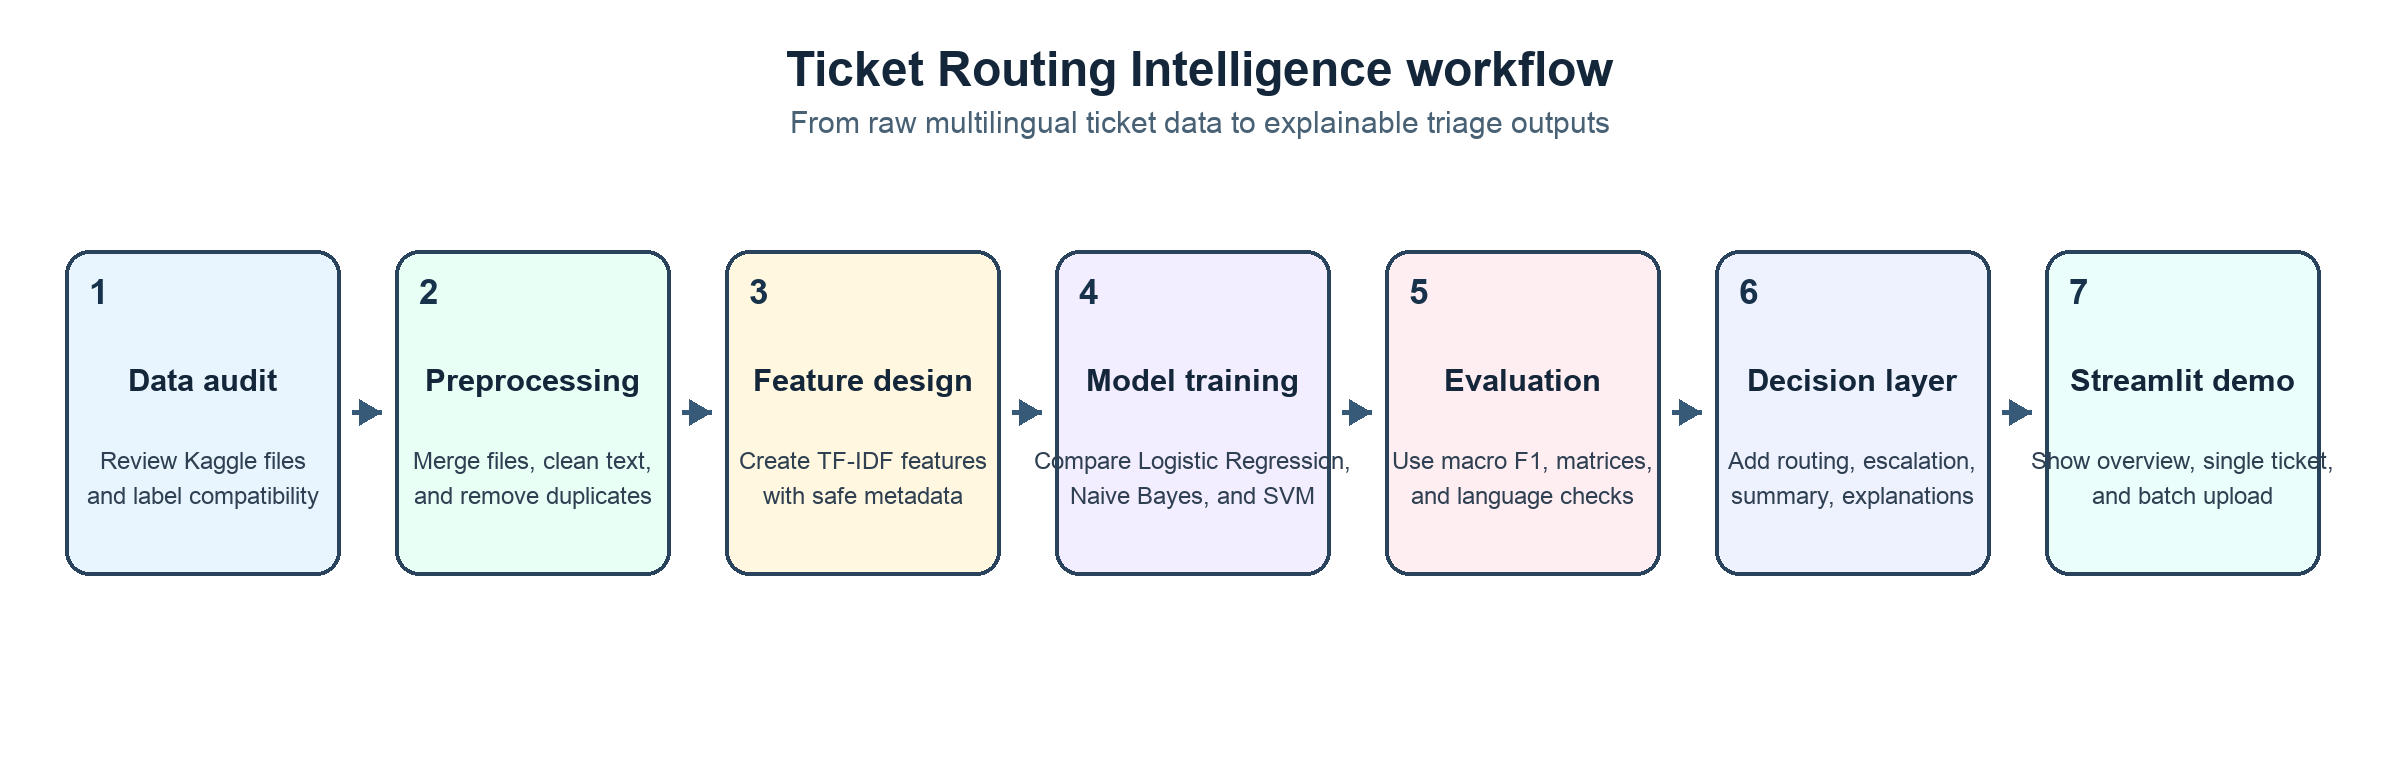
\includegraphics[width=0.98\linewidth]{workflow_diagram_report.png}
\caption{Project workflow used in the final prototype.}
\end{figure}

\subsection{Data Collection and Preprocessing}
The dataset was downloaded from Kaggle. The compatible files were:
\begin{itemize}
  \item \texttt{aa\_dataset-tickets-multi-lang-5-2-50-version.csv}
  \item \texttt{dataset-tickets-multi-lang-4-20k.csv}
  \item \texttt{dataset-tickets-multi-lang3-4k.csv}
\end{itemize}
The two German-normalized files were audited but excluded from the main supervised model because their queue/category taxonomy was different.

The pipeline normalises column names, combines subject and body into \texttt{ticket\_text}, removes duplicate subject-body pairs, and removes rows without usable text. It excludes the \texttt{answer} field because this field is written after a support agent responds. Using it would create target leakage because the information would not be available at ticket creation time.

\subsection{Feature Engineering}
The main feature is \texttt{model\_text}. It combines cleaned ticket text with safe metadata tokens such as type, language, and tags. The cleaning process lowercases text, masks emails and phone numbers, replaces long numbers, removes URLs, and keeps simple alphanumeric tokens. TF-IDF uses unigrams and bigrams with a maximum of 30,000 features.

\subsection{Model Design and Algorithmic Approach}
The project trains two separate supervised tasks:
\begin{itemize}
  \item queue/category prediction using the dataset queue label;
  \item priority prediction using the dataset priority label.
\end{itemize}
For each task, three models were compared: Logistic Regression, Multinomial Naive Bayes, and Linear SVM. The data was split into training, validation, and test sets. Candidate models were selected using validation macro F1. The selected model was retrained on training plus validation data, then evaluated on the held-out test set.

\subsection{Integration of AI Paradigms}
The final prototype integrates supervised learning, probabilistic baseline modelling, symbolic rules, explainability, template summarisation, and transformer comparison. This satisfies the requirement to show more than one AI paradigm. However, only the stable and explainable TF-IDF Linear SVM pipeline is used for live predictions.

\subsection{Design Decisions vs Implementation Details}
A key design decision was to prioritise reproducibility and explainability. The app does not call an external LLM. The summary is template-based, and the explanation is based on TF-IDF terms. This choice reduces cost, privacy risk, and dependency risk. Another decision was to display transformer benchmark results in the app Overview tab, but not to use them for routing.

\section{Empirical Analysis and Results}
\subsection{Experimental Setup}
The final modelling frame contains 44,275 rows. The pipeline uses a train/validation/test approach with stratification when possible. The same random seed is used for reproducibility. Metrics are saved in the \texttt{results/} folder and charts are saved in \texttt{report\_assets/}.

\subsection{Dataset Description}
The data includes multilingual support tickets across English, German, Spanish, French, and Portuguese. English and German dominate the dataset. The dataset includes multiple support queues, including Billing and Payments, Product Support, Technical Support, Customer Service, Service Outages and Maintenance, Returns and Exchanges, Sales and Pre-Sales, Human Resources, and General Inquiry.

\begin{figure}[H]
\centering
\begin{subfigure}{0.86\linewidth}
\centering
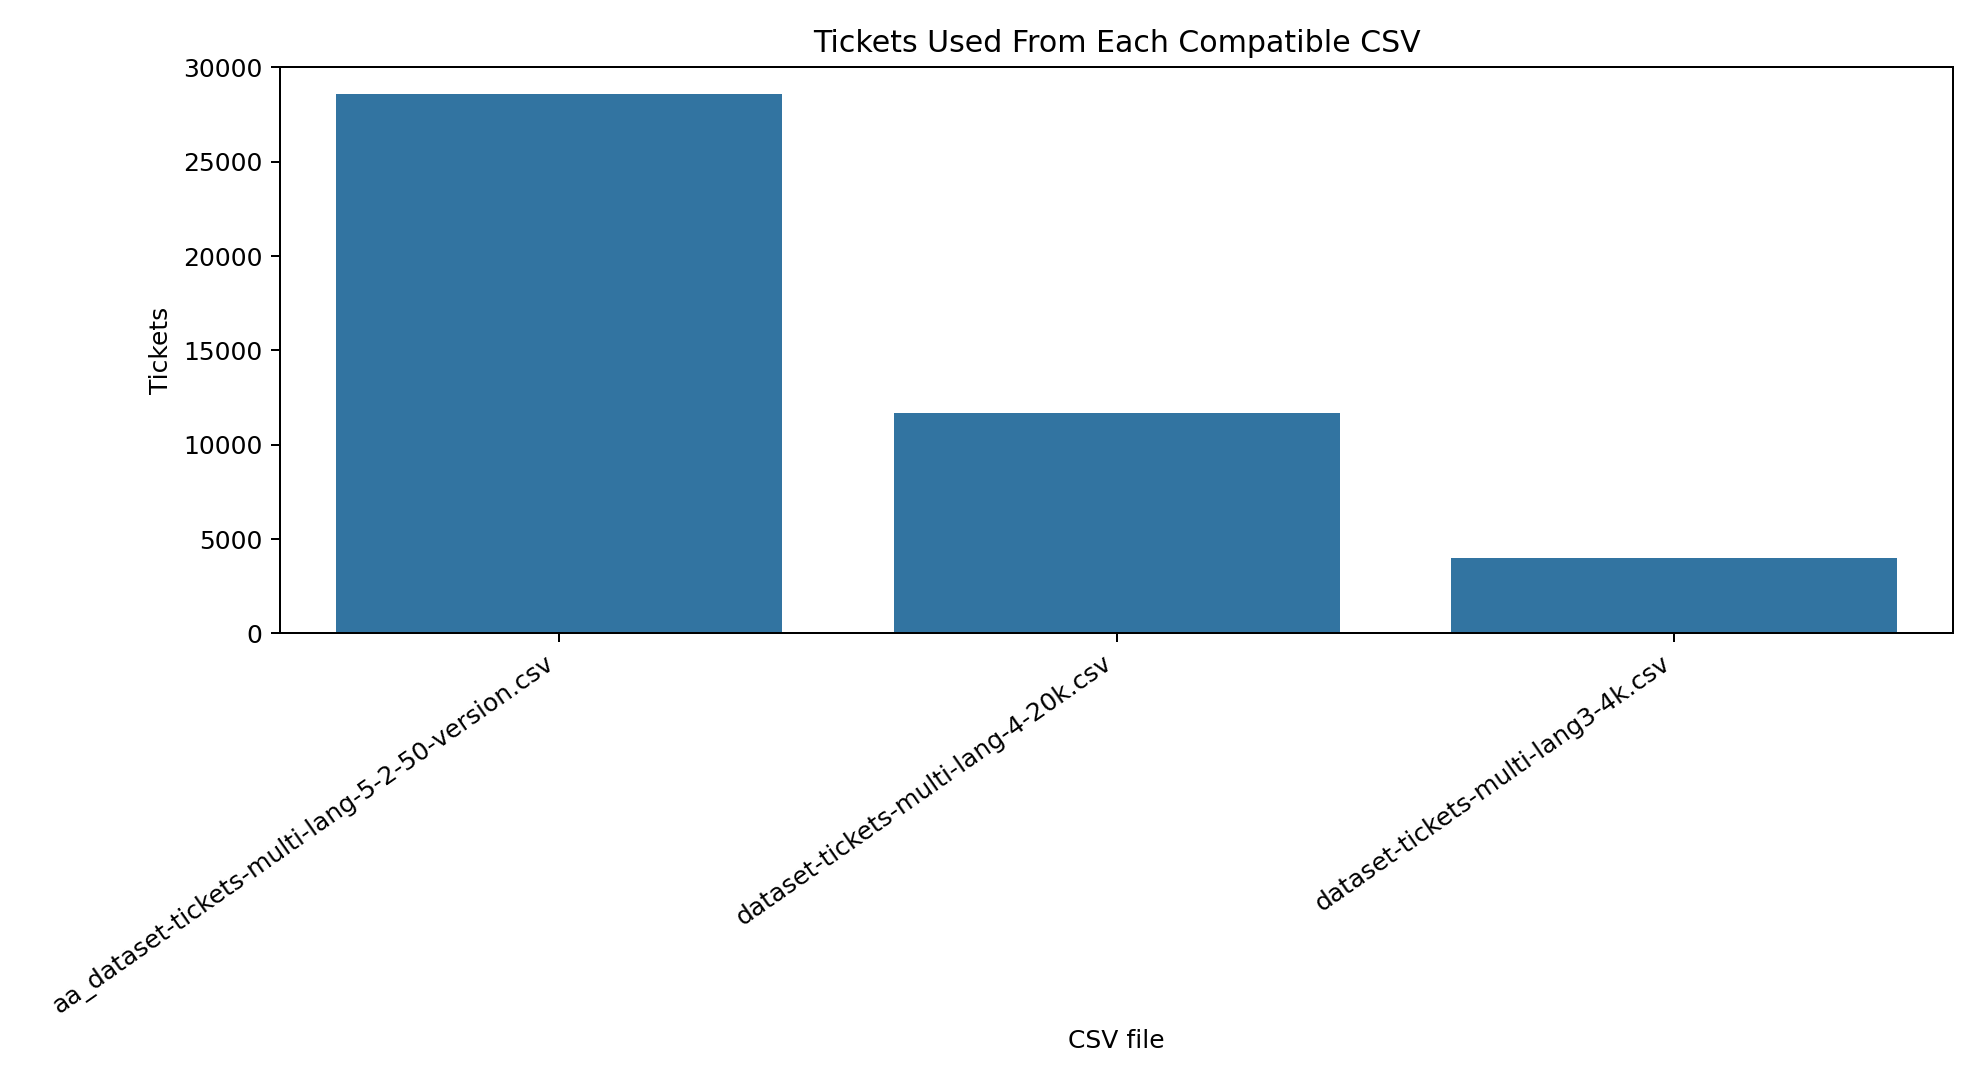
\includegraphics[width=\linewidth]{dataset_file_rows.png}
\caption{Rows contributed by each compatible Kaggle CSV file.}
\end{subfigure}
\vspace{0.5em}
\begin{subfigure}{0.86\linewidth}
\centering
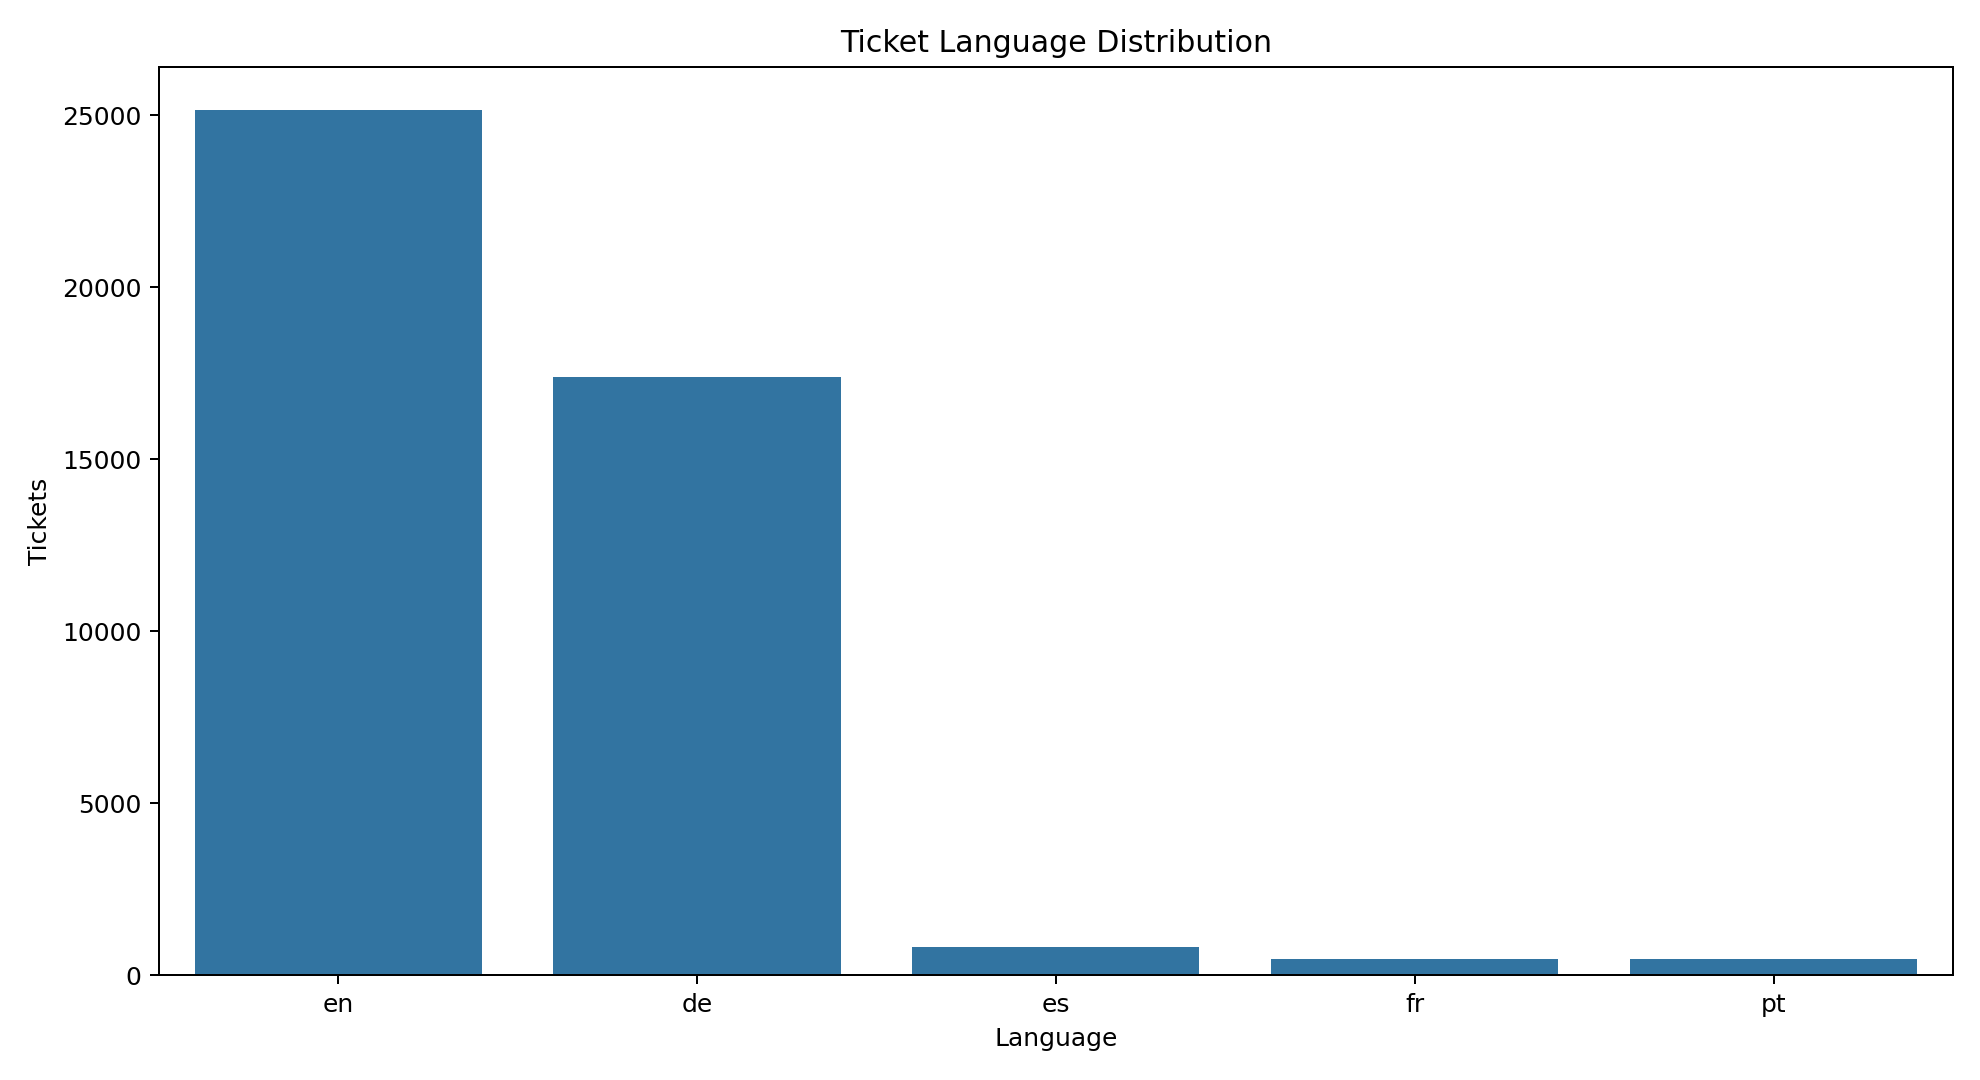
\includegraphics[width=\linewidth]{language_distribution.png}
\caption{Ticket language distribution after preprocessing.}
\end{subfigure}
\caption{Dataset composition used by the final modelling pipeline.}
\end{figure}

\begin{figure}[H]
\centering
\begin{subfigure}{0.78\linewidth}
\centering
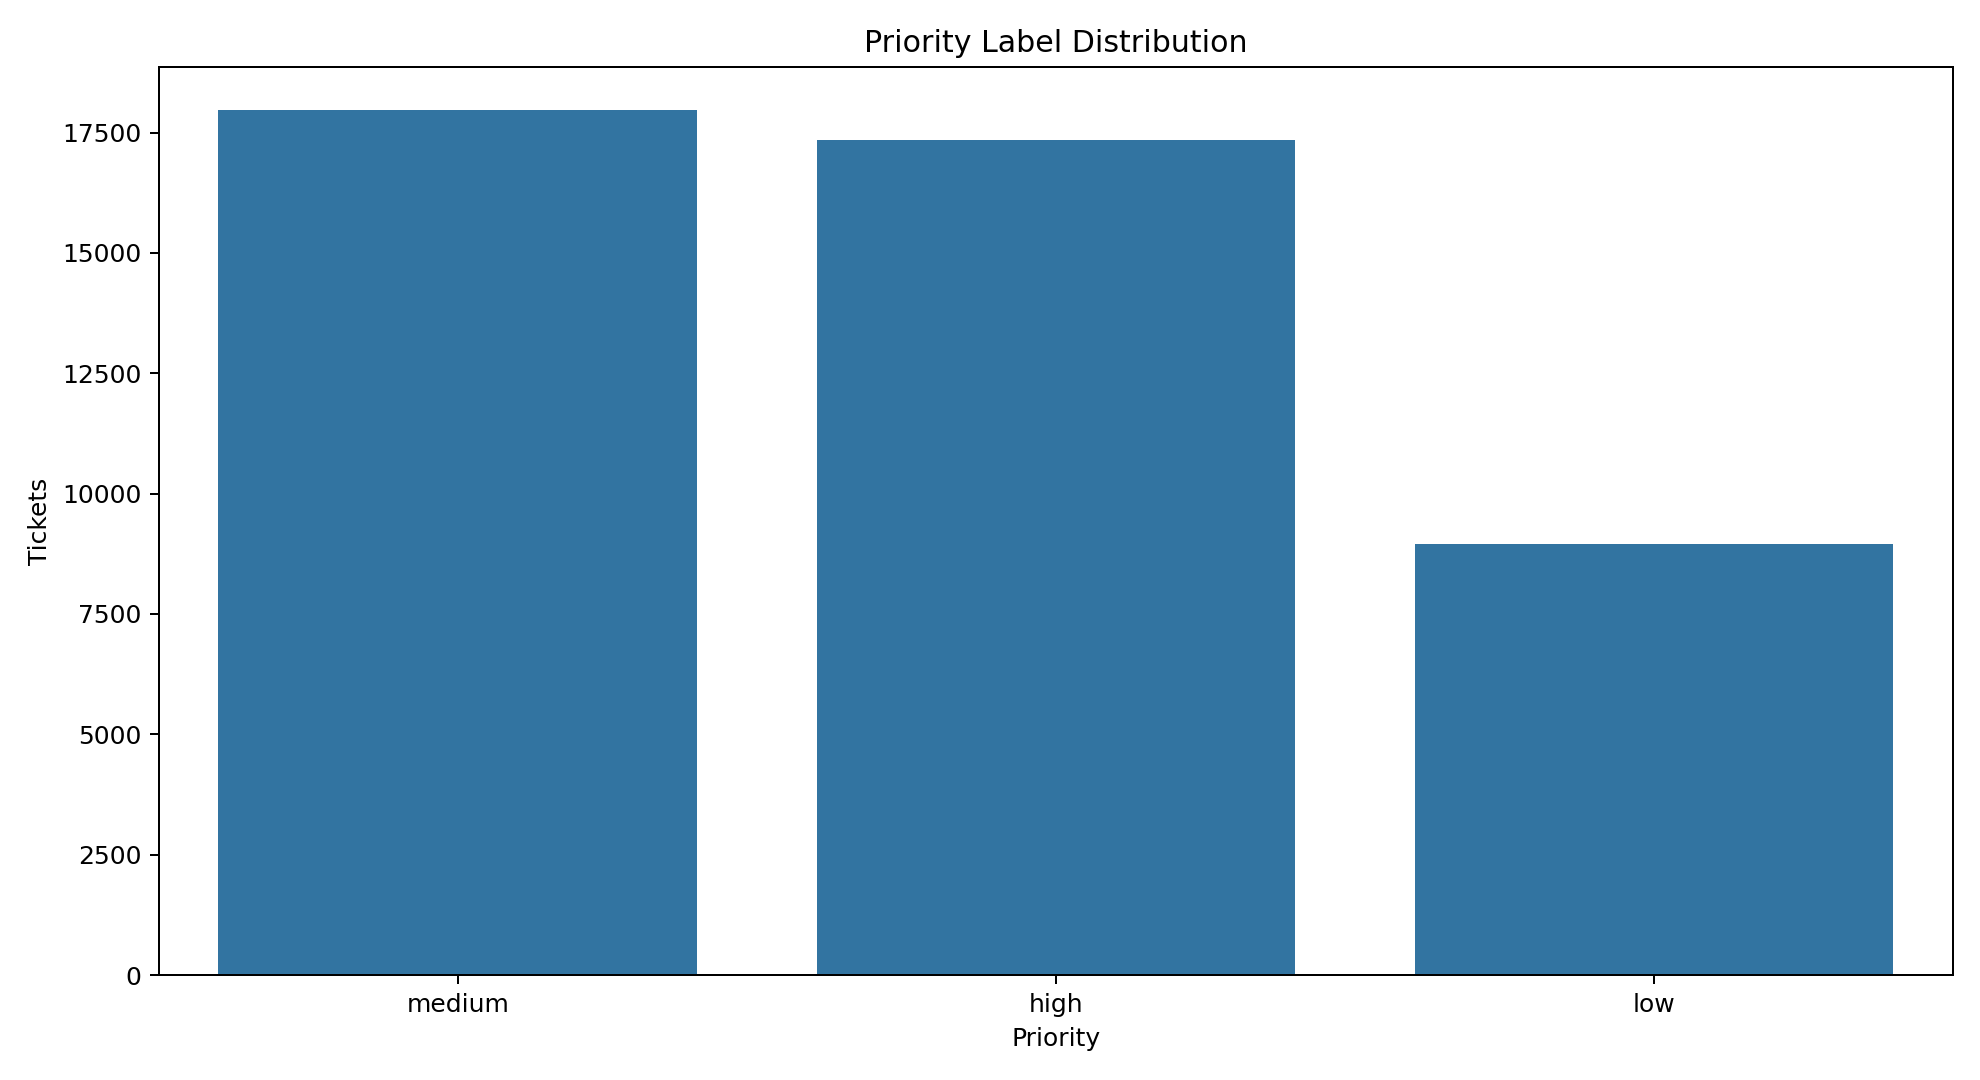
\includegraphics[width=\linewidth]{priority_distribution.png}
\caption{Priority distribution.}
\end{subfigure}
\vspace{0.5em}
\begin{subfigure}{0.86\linewidth}
\centering
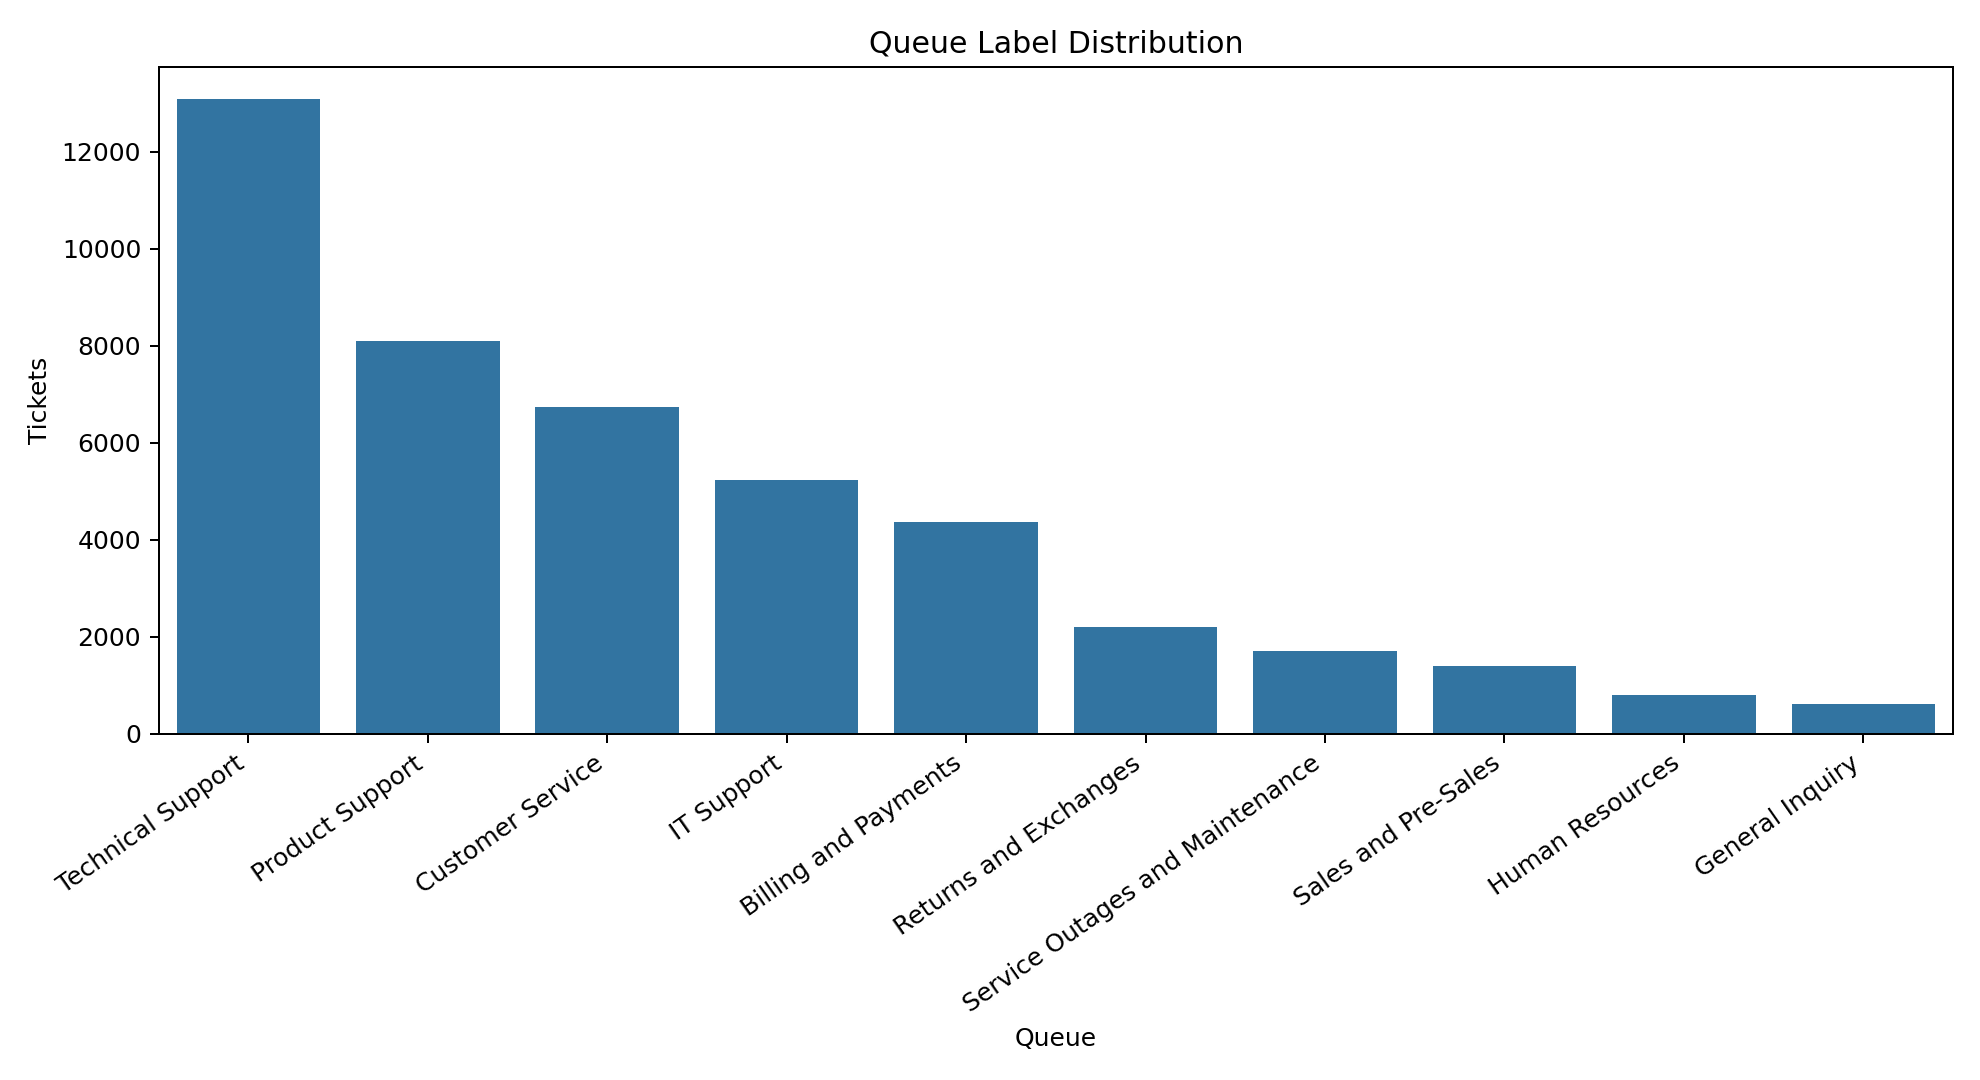
\includegraphics[width=\linewidth]{queue_distribution.png}
\caption{Queue/category distribution.}
\end{subfigure}
\caption{Target-label distributions for priority and queue prediction.}
\end{figure}

\subsection{Evaluation Metrics}
The project reports accuracy, macro precision, macro recall, macro F1, and weighted F1. Macro F1 is the main model-selection metric because it gives equal importance to each class. This is important for imbalanced datasets because a model should not only optimise performance on majority classes.

\subsection{Results}
\begin{table}[H]
\centering
\small
\begin{tabularx}{\linewidth}{lYlrrrr}
\toprule
\textbf{Task} & \textbf{Model} & \textbf{Split} & \textbf{Accuracy} & \textbf{Macro P} & \textbf{Macro R} & \textbf{Macro F1}\\
\midrule
Category & Linear SVM & Test & 0.531 & 0.507 & 0.547 & 0.525\\
Priority & Linear SVM & Test & 0.581 & 0.567 & 0.569 & 0.568\\
Category & Transformer + LR & Sampled & 0.272 & 0.249 & 0.293 & 0.235\\
Priority & Transformer + LR & Sampled & 0.357 & 0.359 & 0.359 & 0.350\\
\bottomrule
\end{tabularx}
\normalsize
\caption{Main test results and optional transformer benchmark results.}
\end{table}

\begin{figure}[H]
\centering
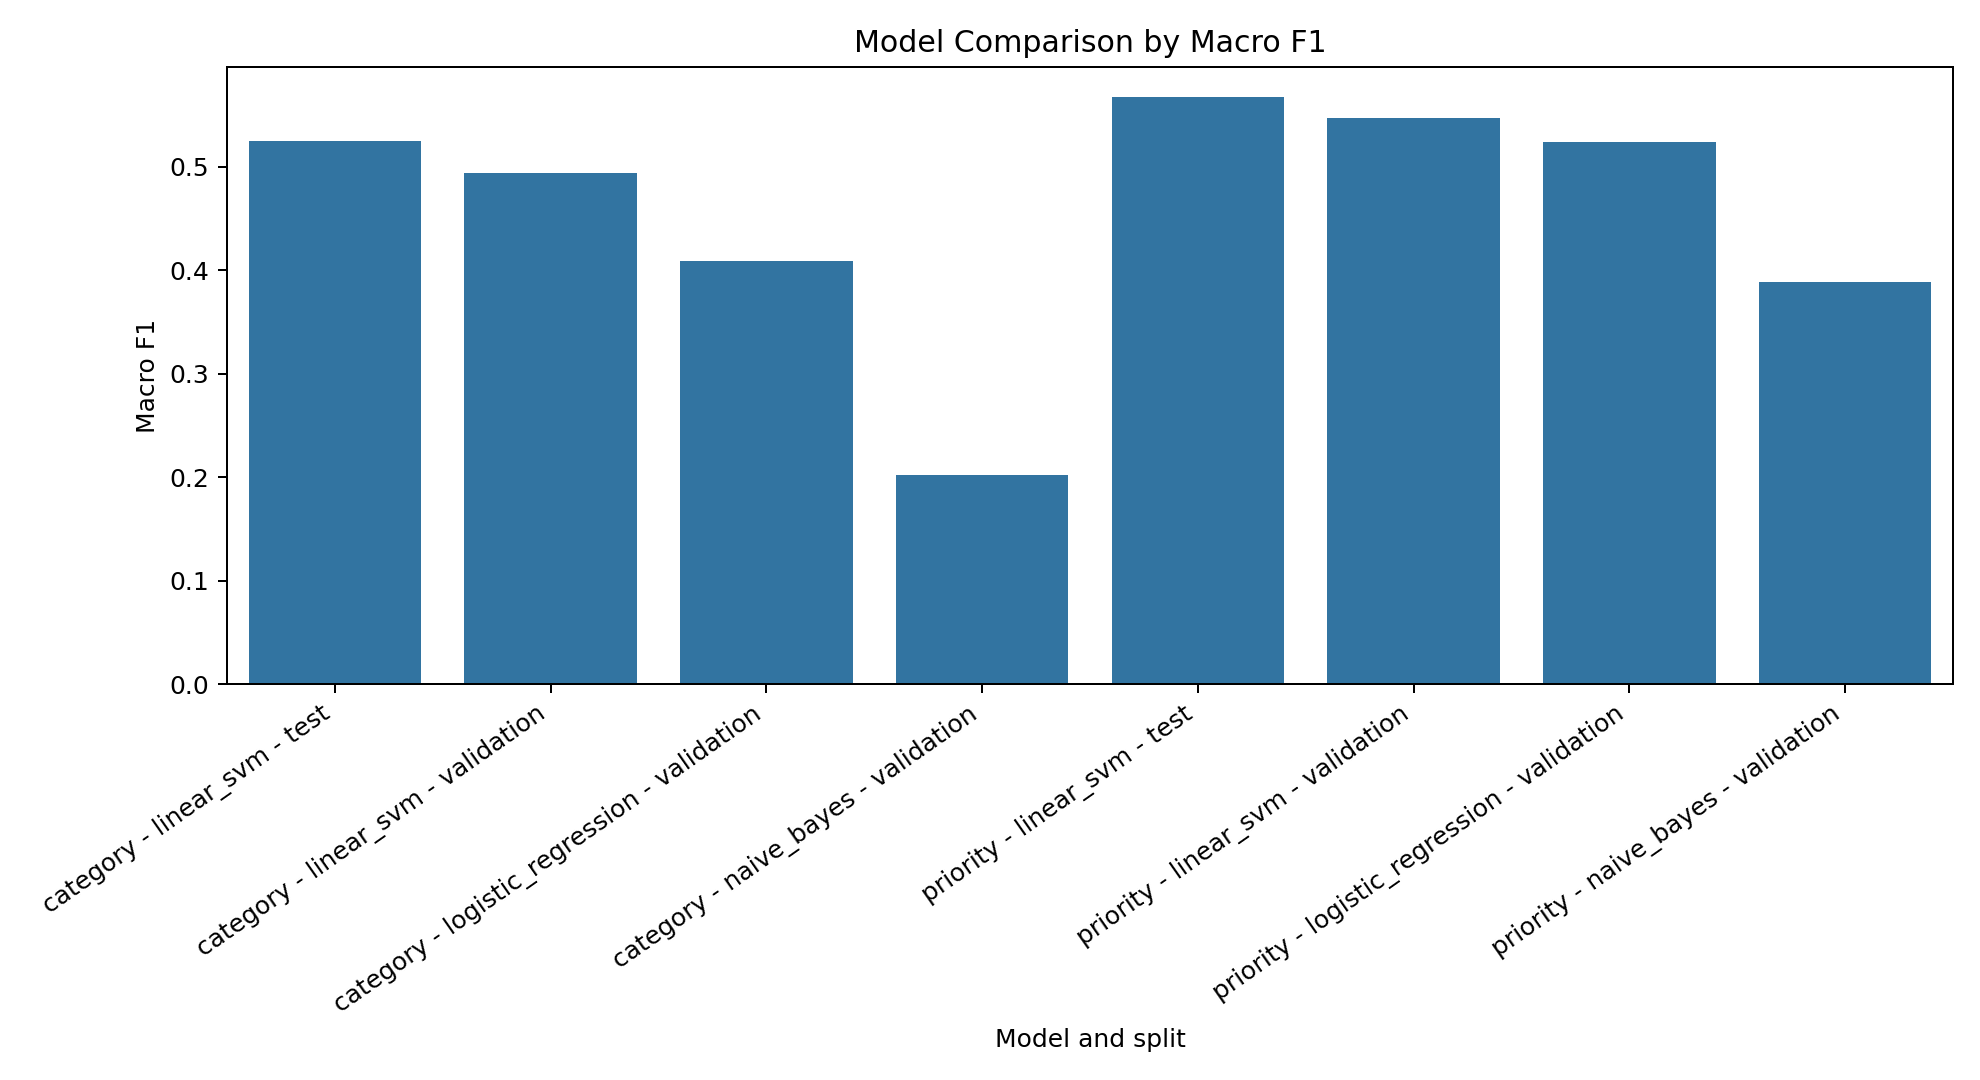
\includegraphics[width=0.94\linewidth]{model_comparison_macro_f1.png}
\caption{Validation and test macro F1 comparison for the main models.}
\end{figure}

\subsection{Transformer Benchmark Results}
The optional transformer benchmark was run on a reproducible sample of 2,500 tickets. The dense embeddings were generated with multilingual MiniLM and classified with Logistic Regression. The category model reached 0.235 sampled macro F1, and the priority model reached 0.350 sampled macro F1. These results were lower than the full-data TF-IDF Linear SVM results: 0.525 macro F1 for category and 0.568 macro F1 for priority.

\begin{table}[H]
\centering
\small
\begin{tabularx}{0.92\linewidth}{lYrr}
\toprule
\textbf{Task} & \textbf{Representation and classifier} & \textbf{Macro F1} & \textbf{Accuracy}\\
\midrule
Category & TF-IDF + Linear SVM, full test set & 0.525 & 0.531\\
Category & Multilingual MiniLM embeddings + Logistic Regression, sampled test & 0.235 & 0.272\\
Priority & TF-IDF + Linear SVM, full test set & 0.568 & 0.581\\
Priority & Multilingual MiniLM embeddings + Logistic Regression, sampled test & 0.350 & 0.357\\
\bottomrule
\end{tabularx}
\normalsize
\caption{Direct report comparison between the deployed TF-IDF model and the optional transformer benchmark.}
\end{table}

The transformer result does not mean that transformers are unsuitable for this problem. It means that this specific sampled and lightly tuned experiment did not outperform the simpler pipeline. A stronger transformer setup would need more data, careful class balancing, hyperparameter tuning, and possibly a classifier better matched to embeddings. For the current assignment, the result supports a responsible technical choice: keep Linear SVM for live prediction and discuss transformer embeddings as validated future work.

\subsection{Result Interpretation and Discussion}
The results show useful predictive signal but also important limitations. Billing and Payments is the strongest category because billing tickets have distinctive vocabulary. Service Outages and Maintenance also performs relatively well. Product Support, IT Support, and Customer Service are harder because their wording overlaps. Priority prediction performs slightly better than category prediction, but low priority remains weaker than high and medium.

Language analysis shows a performance gap. English category macro F1 is 0.604, while German category macro F1 is 0.400. This suggests that future work should improve multilingual preprocessing, use more balanced training data, or tune multilingual embeddings more carefully.

\begin{figure}[H]
\centering
\begin{subfigure}{0.82\linewidth}
\centering
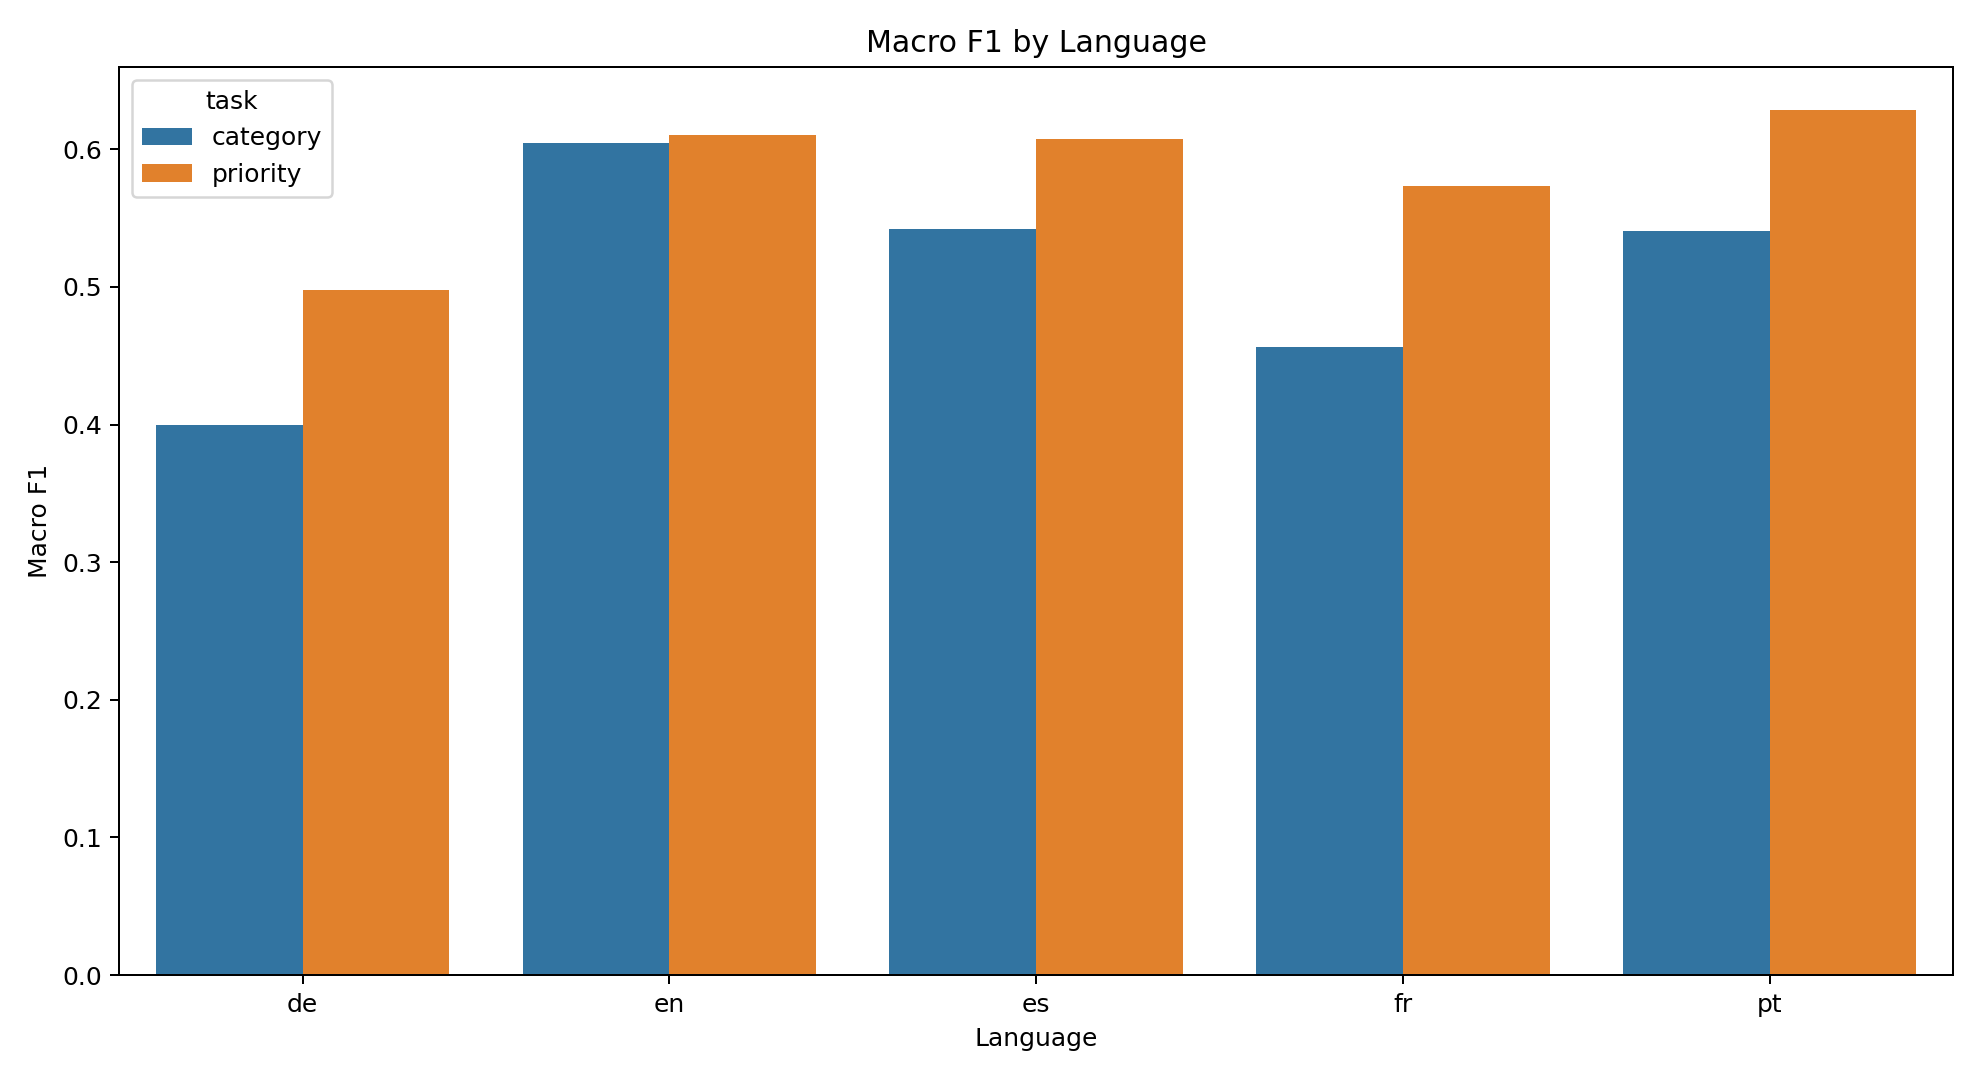
\includegraphics[width=\linewidth]{per_language_macro_f1.png}
\caption{Macro F1 by language and task.}
\end{subfigure}
\vspace{0.5em}
\begin{subfigure}{0.82\linewidth}
\centering
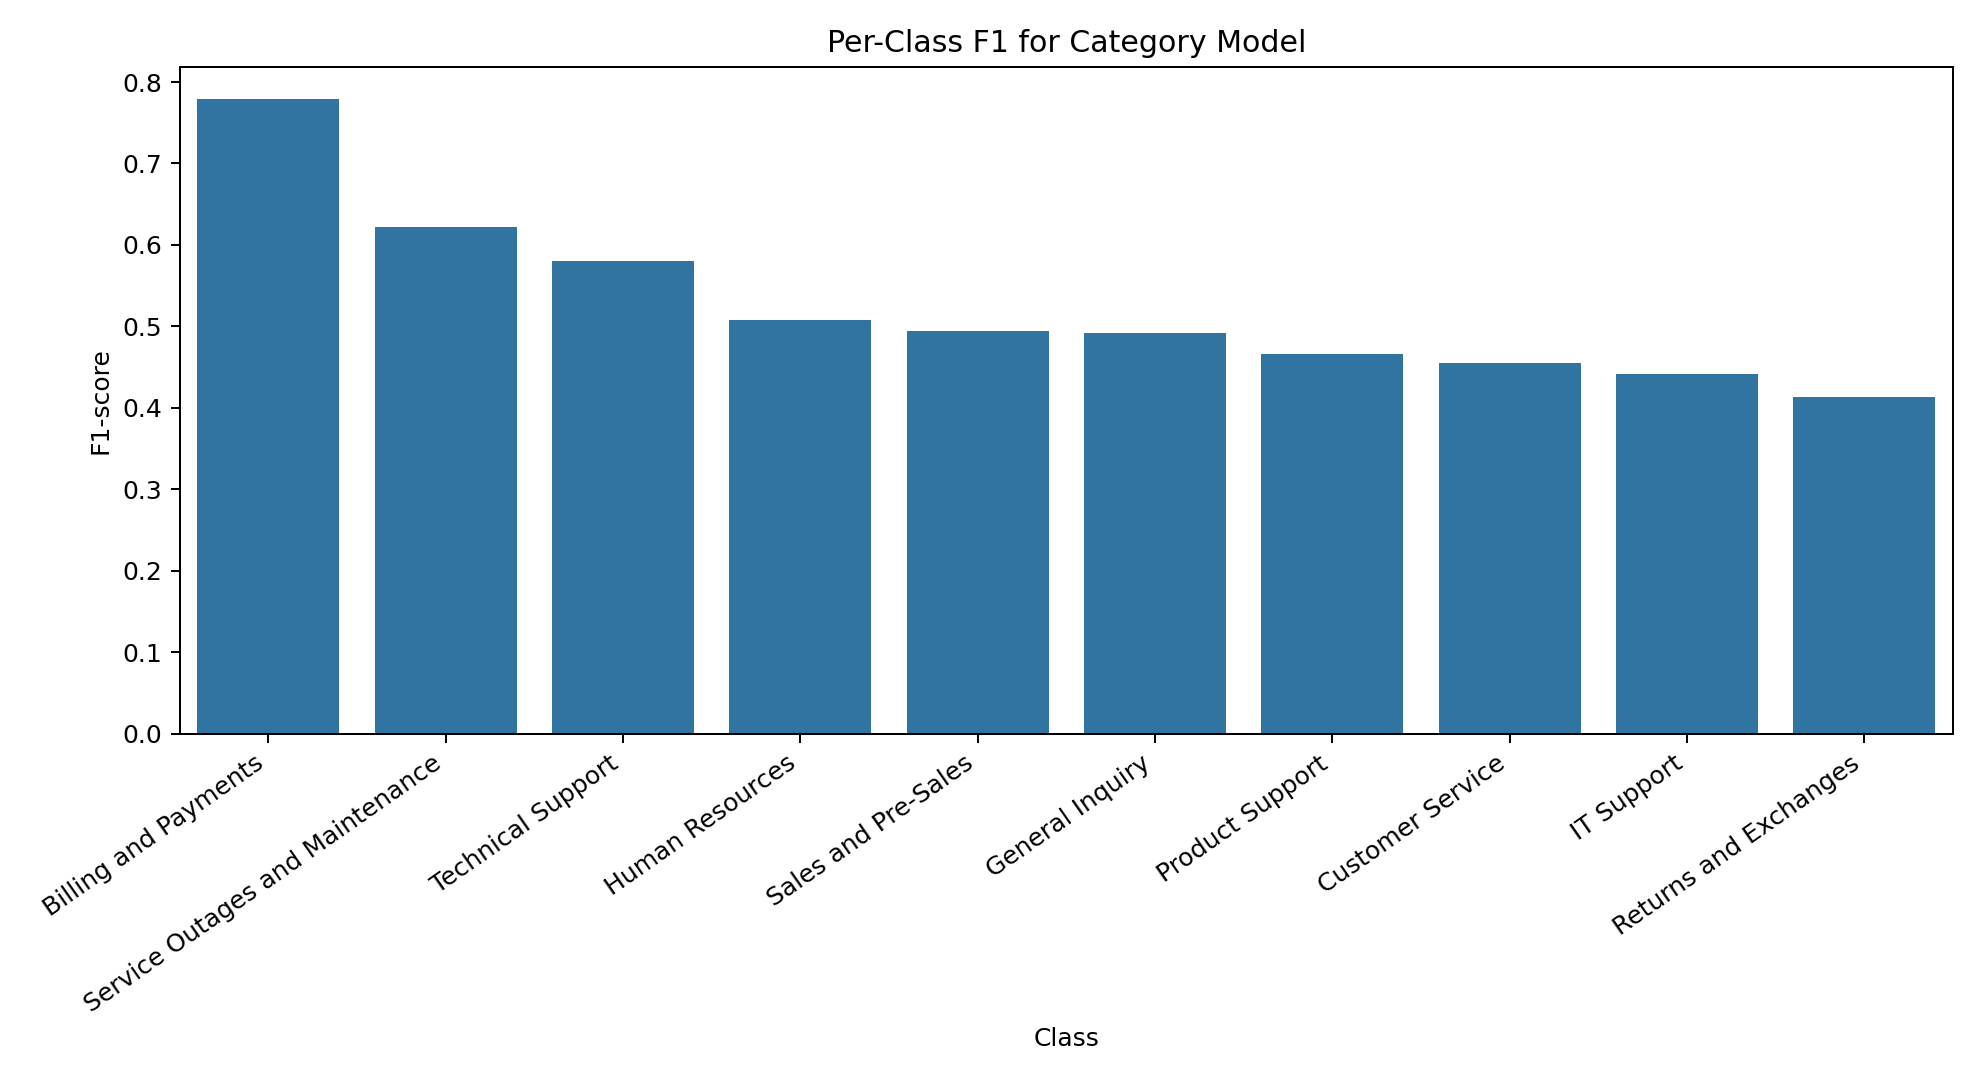
\includegraphics[width=\linewidth]{per_class_f1_category.png}
\caption{Per-class category F1.}
\end{subfigure}
\caption{Detailed performance views used for critical reflection.}
\end{figure}

\section{Critical Reflection}
\subsection{Limitations of the Approach}
The first limitation is moderate macro F1. The model is useful for support, but not for automatic final decisions. The second limitation is language imbalance. The third limitation is the training/inference mismatch: training uses text plus safe metadata, while a manually pasted ticket in the app mainly provides text. Batch files can include richer columns, but single-ticket mode is simpler. The fourth limitation is privacy masking. The app masks obvious emails and phone numbers, but it does not detect all personal information.

\subsection{Failure Cases}
Some tickets are ambiguous. A security-related issue may still mention billing details and be predicted as Billing and Payments. In that case, the model queue and the recommended team can be different. This is expected because queue prediction is learned from labels, while team recommendation also uses security terms. This is a useful design feature, but it must be explained to users.

\subsection{Trade-offs}
The main trade-off is explainability versus complexity. TF-IDF Linear SVM is simple, fast, and explainable. Transformer embeddings can capture deeper semantic meaning, but in this sampled benchmark they performed worse and required heavier dependencies. LLM summarisation could create more natural summaries, but it would add privacy, cost, and reproducibility concerns.

\subsection{Scalability and Computational Constraints}
The current prototype runs locally and uses saved model files. A production version would need an API, authentication, logging, monitoring, drift detection, retraining, and integration with a ticketing platform. The transformer benchmark was limited by sample size and compute. Larger experiments may need better hardware or cloud resources.

\subsection{Alternative Methods and Improvements}
Future work should include confidence calibration, active learning from agent corrections, Unicode-aware multilingual preprocessing, stronger PII redaction, SLA-aware escalation, and better multilingual transformer experiments. A text-only model could also reduce the training/inference mismatch for single-ticket mode.

\section{GitHub Repository}
\subsection{Repository Link}
The GitHub repository is:
\begin{center}
\url{https://github.com/ETHLOB/trn-uts-aipa}
\end{center}

\subsection{Instructions to Run the Project}
Create and install the environment:
\begin{verbatim}
python -m venv .venv
.\.venv\Scripts\python.exe -m pip install -r requirements.txt
.\.venv\Scripts\python.exe -m pip install -e .
\end{verbatim}

Download the Kaggle files:
\begin{verbatim}
.\.venv\Scripts\python.exe -m customer_support_ai.download_data
\end{verbatim}

Train and evaluate the models:
\begin{verbatim}
.\.venv\Scripts\python.exe -m customer_support_ai.train
.\.venv\Scripts\python.exe -m customer_support_ai.report_assets
\end{verbatim}

Run the Streamlit app:
\begin{verbatim}
.\.venv\Scripts\streamlit.exe run app/streamlit_app.py
\end{verbatim}

Optional transformer benchmark:
\begin{verbatim}
.\.venv\Scripts\python.exe -m pip install -r requirements-transformer.txt
.\.venv\Scripts\python.exe -m customer_support_ai.transformer_benchmark --sample-size 2500
\end{verbatim}

\section{Conclusion}
\subsection{Summary of Findings}
This project built a working AI decision-support prototype for customer support triage. It uses a real multilingual dataset, reproducible preprocessing, supervised model comparison, held-out evaluation, routing rules, escalation logic, explanation terms, and a Streamlit dashboard.

\subsection{Key Insights}
The strongest current approach is TF-IDF with Linear SVM. It gives moderate but useful performance and supports explainability. The results are strongest where categories have clear vocabulary and weaker where categories overlap or language representation is limited. The optional transformer benchmark did not improve performance in the current setup, so the final design keeps the simpler model for live predictions.

\subsection{Future Work}
Future work should improve multilingual handling, add confidence scores, learn from human corrections, strengthen privacy redaction, and test more transformer or neural methods under fairer conditions. Production deployment would also need monitoring, data governance, and integration with support systems.

\section{Individual Contributions}
The table below summarises the individual contributions using repository history, presentation artefacts, and the WhatsApp discussion. Contributions that were discussed but are not present in the current main repository are marked as pending evidence.

\small
\begin{longtable}{>{\raggedright\arraybackslash}p{0.18\linewidth} >{\raggedright\arraybackslash}p{0.39\linewidth} >{\raggedright\arraybackslash}p{0.33\linewidth}}
\toprule
\textbf{Member} & \textbf{Confirmed contribution in repository or local artefacts} & \textbf{Pending contribution evidence}\\
\midrule
\endfirsthead
\toprule
\textbf{Member} & \textbf{Confirmed contribution in repository or local artefacts} & \textbf{Pending contribution evidence}\\
\midrule
\endhead
Tumadhir Alsharhan \newline ID: 25605852 & Led the development of the main customer support AI pipeline, including notebooks 01--05, reusable Python modules, Streamlit app, README, run checklist, result files, charts, and demo examples. Amal Maawadh supported these tasks through project planning and presentation/report framing. Tumadhir also prepared and updated group presentation material and Q\&A guidance. & Confirmed in repository history, WhatsApp evidence, and presentation artefacts.\\
\addlinespace
Mario Rubiano \newline ID: 24900627 & Reviewed the codebase, notebooks, app, outputs, and assignment requirements. Added executed notebook evidence and a status/gap report. Implemented the optional transformer-embedding benchmark, result files, notebook 06, transformer dependency file, README/checklist updates, and Streamlit display of transformer benchmark results. Prepared the Speaker 6 responsible AI and future work content. & Confirmed in repository history and presentation artefacts.\\
\addlinespace
Andres Ethorimn \newline ID: 26029165 & Created the original repository/template, shared GitHub access, maintained the main branch, merged pull requests, cleaned data and presentation files from main, restored result artefacts, and reviewed Mario's PR before adding features to main. Presented empirical results in the slide notes. & Confirmed in repository history, WhatsApp evidence, and presentation artefacts.\\
\addlinespace
Amal Maawadh \newline ID: 25605864 & Supported Tumadhir in the main project planning and implementation direction. Shared a detailed implementation plan covering the dataset, AI workflow, models, evaluation metrics, demo features, and HD-level requirements. Drafted presentation content and speaker notes. Presentation artefacts show Amal as Speaker 1 for the project introduction and problem framing. & Confirmed by WhatsApp evidence and presentation artefacts.\\
\addlinespace
Laura Pacheco \newline ID: 25940875 & Presentation artefacts show Laura as Speaker 2 for the solution overview, dataset explanation, and leakage-control explanation. WhatsApp evidence also indicates that Laura explored EDA responsibilities and later experimented with an MLP priority model and an RL routing agent. & \pending{Laura Pacheco: the MLP Neural Network and RL Routing Agent are mentioned in chat, but no corresponding code or results are present in current main repository content. Add branch output or keep this item as future/pending work.}\\
\addlinespace
Carl Lazarus \newline ID: 12043485 & Presentation artefacts show Carl as Speaker 3 for the AI methods section. WhatsApp evidence also indicates that Carl added a demo slide/video and refined the demo wording for the presentation. & \pending{Carl Lazarus: the LLM AI assistant for ticket submission is mentioned as branch work in chat, but no corresponding code is present in current main repository content. Add branch output or keep this item as future/pending work.}\\
\bottomrule
\end{longtable}
\normalsize

\section{References}
\begin{enumerate}
  \item Cortes, C. and Vapnik, V. (1995). Support-vector networks. \textit{Machine Learning}, 20, 273--297.
  \item Joachims, T. (1998). Text categorization with support vector machines: learning with many relevant features. \textit{ECML}.
  \item McCallum, A. and Nigam, K. (1998). A comparison of event models for Naive Bayes text classification. \textit{AAAI Workshop on Learning for Text Categorization}.
  \item Ramos, J. (2003). Using TF-IDF to determine word relevance in document queries. \textit{Proceedings of the First Instructional Conference on Machine Learning}.
  \item Reimers, N. and Gurevych, I. (2019). Sentence-BERT: Sentence embeddings using Siamese BERT-networks. \textit{EMNLP-IJCNLP}.
  \item scikit-learn developers. (2026). scikit-learn: Machine Learning in Python. \url{https://scikit-learn.org/}
  \item Streamlit developers. (2026). Streamlit documentation. \url{https://docs.streamlit.io/}
  \item Kaggle. (2026). Multilingual Customer Support Tickets dataset. \url{https://www.kaggle.com/datasets/tobiasbueck/multilingual-customer-support-tickets}
\end{enumerate}

\end{document}
